\documentclass[sigconf]{acmart}

\usepackage{hyperref}

%\usepackage{endfloat}
%\renewcommand{\efloatseparator}{\mbox{}} % no new page between figures

\usepackage{booktabs} % For formal tables

\settopmatter{printacmref=false} % Removes citation information below abstract
\renewcommand\footnotetextcopyrightpermission[1]{} % removes footnote with conference information in first column
\pagestyle{plain} % removes running headers


\begin{document}
\title{Sociological Applications of Big Data}


\author{Jeramy Townsley}
\orcid{1234-5678-9012}
\affiliation{%
  \institution{IUPUI}
  \streetaddress{425 University Ave}
  \city{Indianapolis} 
  \state{Indiana} 
  \postcode{46202}
}
\email{jtownsle@indiana.edu}


% The default list of authors is too long for headers}


\begin{abstract}
The social sciences have only recently begun to incorporate big data into their analytic frames, and sociology in particular has been slow to adopt big data approaches.  Of the several barriers that social scientists face, one is that big data  originates from other disciplines, so has definitions of data and methods that are new.  Sociologists are creating their own definitions for big data that are useful for their research purposes.  Further, ethical questions that have long framed scientific research are being explored with this new type of data, as social scientists try to find ways to use data that has to potential to expose private identities, and that typically does not allow for the process of asking for informed consent.
\end{abstract}

\keywords{i523, hid347, social sciences, big data, definitions, ethics, critical data studies}


\maketitle

\section{Introduction}


The social sciences have only recently begun to incorporate big data into their analytic frames.  While it may seem that sociology would be a prime fit for big data given the scope of their discipline--describing and theorizing all of society--there have been relatively few thorough explorations of how to apply big data to sociological analysis, particularly in the top sociology journals.  Despite this, outlets have appeared that have taken a lead role in publishing the overlap in these two fields, and solid work has begun. 

Three issues will be addressed.  First, how rapidly have social scientists been incorporating big data into their research and publishing?  Second, what are sites of overlap between sociology and big data, and how is big data defined in terms of what sociologists study.  Third, what ethical questions have arisen for sociologists about the usage of big data, and how are these issues being addressed?  

\section{Tracking Social Science Use of Big Data}
The use of big data to do social science analysis is relatively new.  Using the Google Scholar index to track specific terms by year creates a picture of the rapidity with which social scientists seem to be exploring big data.  Prior to and inclusive of 2005, Google Scholar had 7,560 records containing the phrase, {\em big data} (excluding patents and citations; retrieved 10/5/2017).  Figure 1 shows the cumulative number of records in Google Scholar from 2005-2016 that contain the phrase {\em big data} plus either {\em sociology} or {\em social science.}  There were only 559 in 2005, a mere 7.4\% of the total {\em big data} references up to that point.  The tipping point seems to be around 2012-2013 when these terms start to appear together.  While after 2015 the number seems to level off, that may simply be an artifact of Google Scholar not yet picking up references since then.  Regardless, there has clearly been a dramatic surge in the last five years.  It is unlikely that all of these represent primary research by social scientists using big data, but it does represent a significant increase in the terms being found in the same articles, implying intersections of interest between the fields.    

The recency of sociology's usage of big data is particularly striking when seen through the sociology-specific database, Proquest's {\em Sociological Abstracts} (Figure 1). There are significantly fewer results, since it only indexes peer-reviewed articles in sociology journals, compared to Google Scholar's results with the diversity of their indexed sources.  From 2005-2016, there were 517 total references to {\em big data} in their 1,800 indexed serials (retrieved 10/7/2017), with almost all of those since 2013--there were only 2 references from 2005-2011.  From what had been indexed as of October 2017, there were already 157 references for that year.    

Academics publishing in the top sociology journals seem not to be using big data techniques with significant regularity.  The ISI Web of Science tracks impact factors for peer-reviewed journals, and those values can be used to create a general (if not somewhat controversial) list of the top journals in any given field.  Based on the impact factors for 2015, the top ten journals in sociology have a total of 92 usages of the term {\em big data}, according to a Google Scholar search (10/5/2017).  This is a total search of any timeframe, and not all of these references represent primary research using big data, but simply refer to the usage of the terms.   The top three journals each have 17 usages of the term, the most of these top ten, while Social Problems contains only 1 reference.  Figure 2 shows these top ten journals along with a count of the usage of the term {\em big data} from the Google Scholar search.  

In contrast, a relatively new journal began publishing in mid-2014 by Sage, Big Data and Society (BDS).  It self-describes as publishing ``interdisciplinary work principally in the social sciences, humanities and computing and their intersections with the arts and natural sciences about the implications of Big Data for societies.''  While primary research using big data in traditional sociology journals is relatively sparse, BDS publishes twice a year, containing primary research, and other relevant discussions, such as ethics and research methods.  Because of its specificity, it is an important resource for the overlap of these fields.

\section{Defining Big Data}
Big data has been described as having velocity, variety, and volume, attributed to Laney in the early 2000s.\cite{japec15}  Kitchin includes five additional concepts: exhaustive in scope, fine-grained resolution, relational, extensional (ability to add fields), and scalable (the latter two concepts sometimes combined under the single concept of flexibility).\cite{kitchin14}  In this analysis, Kitchin argues that big can be differentiated from small data specifically along these eight axes, and that while some small datasets may have characteristics of big data, such as strong relationality or wide variety, there is little overlap along the other axes.   In their 2016 review, Kitchin and McArdle test 26 datasets that have previously been defined as big data for their {\em fit} based on these differentiating concepts.\cite{kitchin16}  They conclude that not only do not all datasets fit all of the criteria Kitchin described, but they also do not all fit the original descriptions of volume, velocity and variety.  However, they do believe that all of the 26 datasets are characterized by velocity and exhaustivity, which they describe concisely as, ``real time flow of data across a whole system'' that produces a large dataset.  The other descriptive concepts are still relevant, and may be pertinent to some big datasets, but not to others.

Others have taken different approaches to understanding what big data is.  Dalton, using a political sociology lens, notes that the size of the dataset is clearly not the defining issue, since administrative data, such as the Census, can easily contain millions of subjects with thousands of variables, and this is not typically classified as {\em big data}.\cite{dalton16}  Instead, he notes that while data like the Census is constructed specifically for the researchers' purposes, {\em big data} is often indirect, having been collected from {\em unconventional sources} and often involves merging several distinct datasets.  In this case, finding similar types of data for cross-national studies can be a challenge, but typically involves finding government, administrative data on similar topics in many countries that have the possibility of being merged for comparative analysis into one dataset.  Similarly, Brayne describes that sociological research shifts the definition away from specific characteristics of the data itself, like the size or speed of the data, but on the various institutional sources from which the data is gathered and then merged, thus emphasizing the process of collection rather than data features.\cite {brayne17}

Connelly, et al, and Japec, et al, discuss the {\em found} nature of big data in sociology, also highlighting the importance of administrative data, and the issues of merging data that was often constructed by different people, in different times, and for different purposes, but that may be similar enough for comparative analysis.\cite {connelly16} \cite {japec15}  Additionally, they note other types of data, particularly social media data, which can describe the real-time behavior of users.  This type of data, unlike surveys, experiments, or other types of {\em researcher constructed-data} was not necessarily ever intended to become research data.  But since sites like Twitter and Facebook collect data from their users and make it available, or when researchers can scrape data directly as it happens, it becomes information that can be re-purposed by social scientists.  Continuing along that line, they describe two types of data--made and found.  The former, which has been the typical source of social science research data, consisting of experimental and observational data, does not typically have the features associated with big data, but is designed to answer specific questions, and is highly systematic.  Found data, on the other hand, whether administrative, or otherwise, is often very messy when it comes to the researcher, and is often not systematic, since it was not intentionally designed to answer a research question.  

Yet another approach to understanding sociological types of big data is to look at the outcome of using it.  In contrast to the previous approaches, which focused on qualities of the data or the way it was produced, Madsen, et al explore how big data functions to change society and the people it impacts.\cite{madsen16}  They look at three aspects of big data using this frame: how it satifies daily life, how it can produce new modes of governance, and how it can be used to predict.  Arguably, all of these have been occurring for a very long time, particularly since governments have been formally collecting data on its citizens.  However, they argue that the large-scale collection of real-time data, and the integration of disparate sources of data has the potential to dramatically intensify these processes.  Brayne highlights each of these concerns with her analysis of the data collection procedures of the LAPD.\cite {brayne17}  She provides the example of ALPR, the automatic license plate reader system, by which cameras from various city sources, including those on police cars, automatically capture all license plate numbers it detects and logs them as geotagged information.   First, mass numbers of citizens' locations, or at least their cars' locations, have been {\em datified}--where they were at a specific time that it was caught on camera.  Second, this represents a novel form of surveillance by the state.  In previous times, people were only logged into a policing system if they had been stopped because they were reasonably suspected of criminal activity.  ALPR represents a wide net being cast to sweep up all people, now placed into policing databases, regardless of legal status of probable cause or consent.  For Brayne, this represents a fundamentally new form of relationship between citizen and state, a new form of governance.  Third, these and other types of data collection techniques have transformed traditional policing models at LAPD to predictive models, in which law enforcement is not simply responding to citizen calls, but generates incentives for the LAPD to invest resources into specific districts that algorithms have determined are more likely to experience criminal activity.  Like the issue of wide-sweeping nets that put citizens into policing databases, predictive policing also represents a new modality of governance, since it directs public funds and interactions between the state and the public.

\section{Ethical Issues of Big Data in the Social Sciences}
These issues lead to the questions that social scientists have raised about the ethics of using big data for research.  After several classic ethical failures on the part of social and medical scientists, such as the Tuskegee syphilis study, Zimbardo's prison study with Stanford college students, and Milgram's electric shock experiment, the scientific community, along with government agencies, came together to create the Belmont Report (1978), outlining fundamental principles of ethical research, as well as providing specific ways to apply those principles.\cite {fiske14}   Each of the principles on their own has proved resilient as a way to plan ethical research with humans: respect for persons, beneficence, and justice.  However, these can be abstract and difficult to conceptualize their application, particularly in boundary or novel situations.  Big data represents such a challenge.  

As Brayne highlights, state usage of big data leads to legal questions about the relationship between the state and citizens.  However, as researchers many of the same issues she raises are relevant.  One of the specified applications of the Belmont Report is the requirement for informed consent from research participants--researchers are expected to fully inform participants of risks and benefits of a study, the goal of the study, assure them they can leave the study at any time, and then get formal consent to include the individual in the study.  However, mass collection of public or administrative data for research purposes almost never follows this guideline.  To balance difficult cases, ethics committees often consider the risks to the participant when ideal protocols cannot be followed.  But these can be difficult to assess, especially in new research territory, with new forms of data.  McFarland, et al, note that privacy and potential harm to those caught up in mass data sweeps are of particular concern. \cite {mcfarland16}

Lazer and Radford discuss these same ethical concerns. \cite {lazer17}  They note that while some of these issues are not new, for example, the common practice of using government administrative data, such as the Census, for research purposes, are largely considered resolved, since strict protocols are in place to prevent any individual from being connected to their specific information.  In that case, while there is no informed consent by the subject for the researcher to use the data, there is little chance for harm to the individual, and little chance for privacy breaches.  The repository of that data, the federal government, is responsible for data security and data de-identification in that case, not the researcher.  Other large datasets, such as surveys implemented by the National Institutes of Health, or the General Social Survey, take similar extraordinary precautions to prevent data breaches that connect survey responses or medical histories to individuals.\cite {lazer17}  On the other hand, the {\em found} nature of big data provides very different challenges.  For example, for data sweeps that pick up Facebook or Twitter data, it may be very easy to connect individuals to information since much of that information is publicly available.  Fiske and Hauser describe recommendations made by most Institutional Review Boards, which includes requiring researchers to specify a privacy-protection plan that has to be registered with the IRB to ensure subject's privacy faces minimal risk of exposure.  Reuse of such data would continue to require identities of subjects to be protected.  Using these types of publicly available data would be classified as {\em excused} research, meaning issues of informed consent would be considered waived, as long as the research subjects' identities were protected. \cite{fiske14}

Several sources point to the need to incorporate {\em critical data studies} into big data research, particularly research that incorporates products of human behavior, like social media or administrative data.  Felt (2016) describes issues of social science research with social media. \cite{felt16}  They note the number of studies that use data from specific sources, specifically Twitter and Facebook, or some combination of those and other sources.  While they note the specific privacy issues of connecting information from individuals across various platforms, they discuss the broader framework that social scientists should employ to think critically about how the data is being used by researchers.  In contrast to previous eras, when data was often considered neutral, Felt argues that the use of social data cannot be considered neutral since it has the capacity to impact the subjects whose data is being used, for the research findings to retroactively come back to the subjects.  Critical Social Theory from the early 1900s builds the foundation for this kind of interrogation of the use of the data, how the data was generated, and the types of research questions that were originally asked that led to this data being used.   For example, they point to the argument that data is inherently political, and urge the researcher to ask whose interests are being served by generating and using this data, and to particularly be sensitive to how inequalities may be maintained or exacerbated by the data.  Further, they ask the researcher to consider broader relationships between the data and society, highlighting the fact that data is never {\em raw}, but is always constructed, even if it is scraped from existing sources, and that the data represents specific power relationships within society.  They urge an orientation that intentionally looks for socially progressive ways to think about and use data.

\section{Conclusion}
Sources and processes of big data are relatively new, and the social sciences are trying to catch up to the new resources they offer, and challenges they pose.  Sociologists, in particular, seem to have only started publishing research using big data in the last five years when a rapid climb becomes evident in the database {\em Sociological Abstracts}.  One task for social scientists is to define what constitutes big data.  Research in physics, such as work to discover the Higgs-Boson, where hundreds of trillions of collisions had to be analyzed, far outpaces the size of data that social scientists would historically have analyzed, and likely continues to be exponentially larger than data they would analyze today.  Sociologists describe administrative data as big data, particularly in the way that disparate datasets may be combined, with the complexity and relationality that entails.  They also describe real-time data such as that collected from social media.  Another early-stage set of questions with which researchers need to grapple are ethical concerns about the subjects they study, and the impact on society of the use of big data research.  The privacy and safety of participants need to be protected, and issues raised by critical data studies urge researchers to ensure that research has a positive impact on those that might otherwise be disenfranchised from social resources.



\begin{figure}
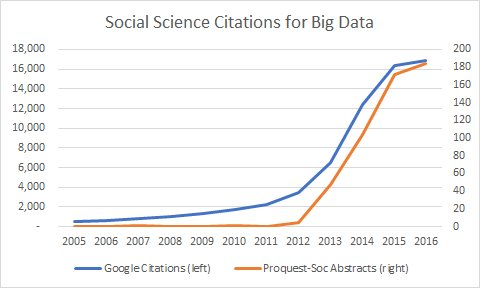
\includegraphics[width=\columnwidth]{images/figure1}
\caption{Citations over time for the phrase Big Data plus sociology or social science in Google Scholar (blue, 10/5/2017) and citations for the phrase Big Data in Proquests's, Sociological Abstracts (orange, 10/7/2017).}
\label{f:figure1}
\end{figure}

\begin{figure}
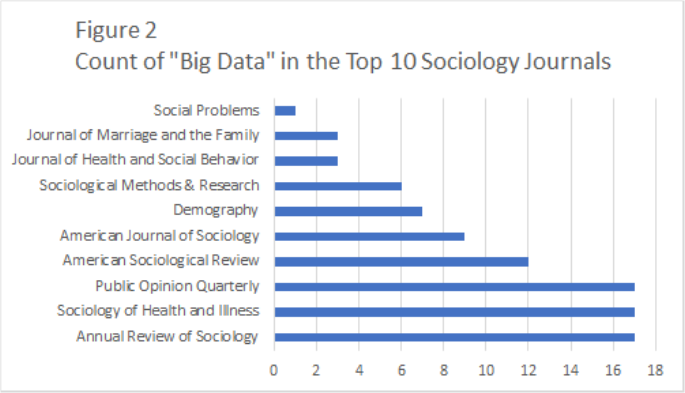
\includegraphics[width=\columnwidth]{images/figure2}
\caption{Count of the phrase Big Data in the top 10 sociology journals.  Google Scholar, 10/5/2017}
\label{f:figure1}
\end{figure}


\bibliographystyle{ACM-Reference-Format}
\bibliography{report} 

\end{document}
